\section{Desarrollo de la práctica}

\subsection{Creación del repositorio}

Se creó el repositorio denominado Git\_Issues en GitHub y se agregaron los integrantes del equipo como colaboradores para permitir el trabajo conjunto.

\textbf{Repositorio utilizado:}

\begin{center}
\texttt{Maria-mtz11/Git\_Issues}
\end{center}

\begin{figure}[H]
\centering
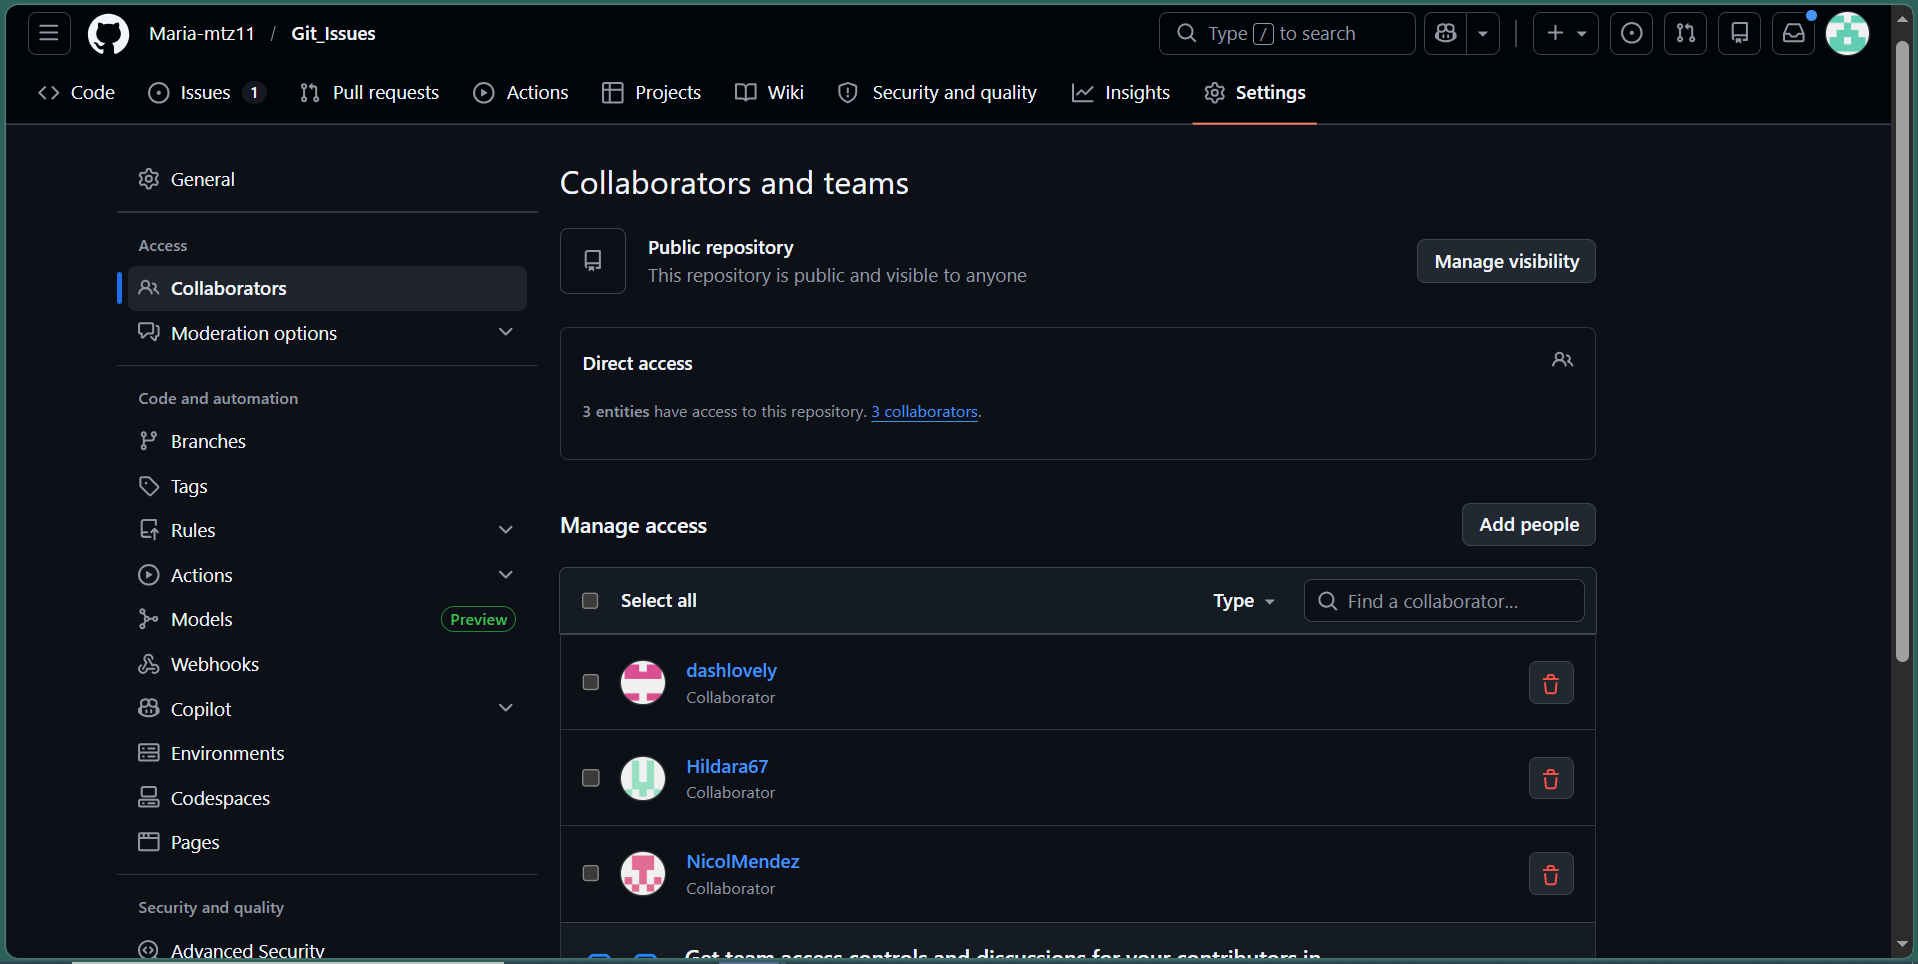
\includegraphics[width=15cm]{imagenes/repositorio.png}
\caption{Repositorio creado en GitHub.}
\label{fig:repositorio}
\end{figure}

\subsection{Creación del Issue}

Se creó un Issue para reportar una problemática detectada dentro del proyecto utilizando GitHub CLI.

\textbf{Título del Issue:}

\begin{quote}
Error en lectura UART
\end{quote}

\textbf{Descripción:}

\begin{quote}
La comunicación serial falla al iniciar el sistema.
\end{quote}

La incidencia fue registrada correctamente en el repositorio, permitiendo documentar el problema y dar inicio al flujo de trabajo colaborativo para su seguimiento y resolución.

\begin{figure}[H]
\centering
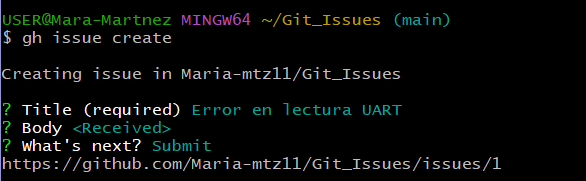
\includegraphics[width=15cm]{imagenes/creación.png}
\caption{Creación del Issue mediante GitHub CLI.}
\label{fig:creacion}
\end{figure}

\subsection{Visualización de Issues}

Para visualizar los Issues registrados se utilizó GitHub CLI mediante el siguiente comando:

\begin{lstlisting}[language=bash]
gh issue list
\end{lstlisting}

Posteriormente se consultó el Issue específico mediante:

\begin{lstlisting}[language=bash]
gh issue view 1
\end{lstlisting}

Esto permitió verificar la información registrada, incluyendo el estado, descripción y responsable de la incidencia.

\begin{figure}[H]
\centering
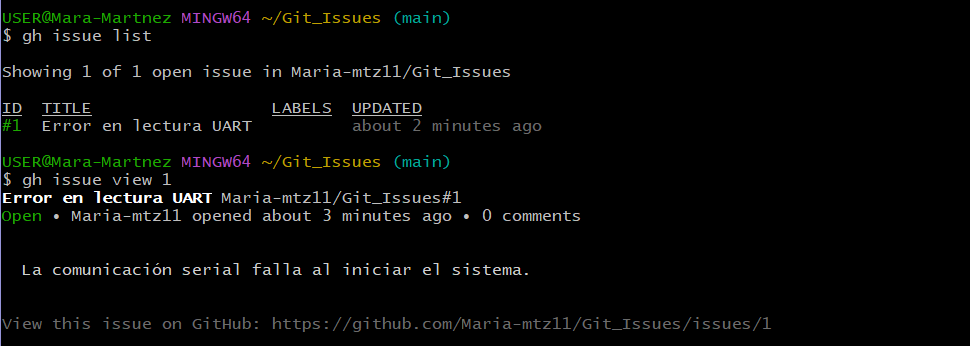
\includegraphics[width=15cm]{imagenes/visualizacion.png}
\caption{Listado y visualización del Issue.}
\label{fig:visualizacion}
\end{figure}

\subsection{Asignación del Issue}

Uno de los integrantes del equipo fue asignado como responsable del Issue para atender la incidencia reportada.

La asignación permitió definir claramente quién sería el encargado de resolver el problema y dar seguimiento a las actividades relacionadas con la incidencia.

\begin{figure}[H]
\centering
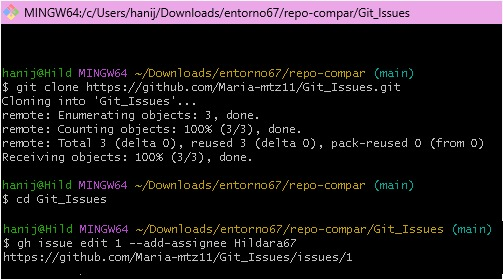
\includegraphics[width=15cm]{imagenes/asignación.jpeg}
\caption{Asignación del Issue a un integrante del equipo.}
\label{fig:asignacion}
\end{figure}

\subsection{Comentarios y seguimiento}

Otro integrante agregó comentarios al Issue para dar seguimiento al avance de la actividad y así mantener comunicación con el resto del equipo.

Ejemplo de comentario realizado:

\begin{quote}
Estoy revisando el problema.
\end{quote}

\begin{figure}[H]
\centering
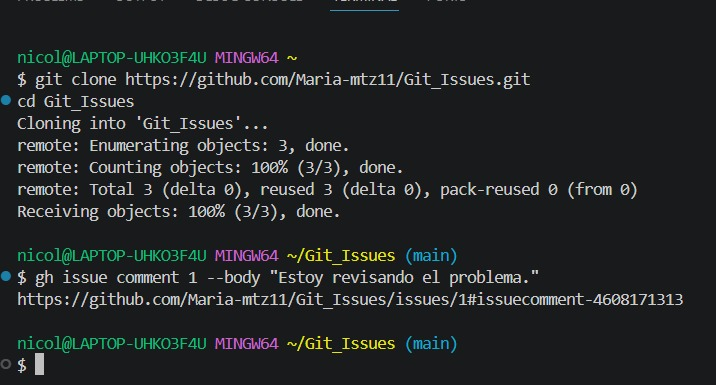
\includegraphics[width=0.9\textwidth]{imagenes/comentario.jpeg}
\caption{Comentario agregado al Issue.}
\label{fig:comentario}
\end{figure}

\subsection{Corrección de la incidencia}

Con el objetivo de simular la resolución de la incidencia reportada, se realizaron modificaciones en el repositorio y posteriormente se registraron los cambios mediante Git.

Para ello se ejecutaron los siguientes comandos:

\begin{lstlisting}[language=bash]
git add README.md
git commit -m "Correccion del issue #1"
git push origin main
\end{lstlisting}

Una vez realizados los cambios, estos fueron almacenados en el historial del repositorio mediante un commit y posteriormente enviados al repositorio remoto para que todos los integrantes del equipo pudieran acceder a la versión actualizada del proyecto.

\begin{figure}[H]
\centering
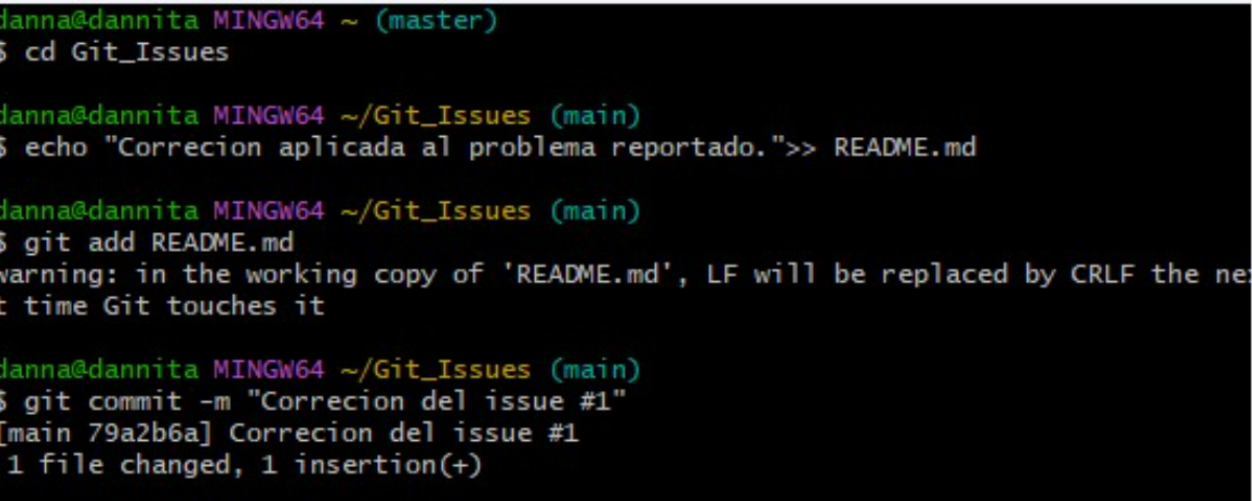
\includegraphics[width=0.9\textwidth]{imagenes/corrección.png}
\caption{Commit realizado para registrar la solución de la incidencia.}
\label{fig:correccion}
\end{figure}

\begin{figure}[H]
\centering
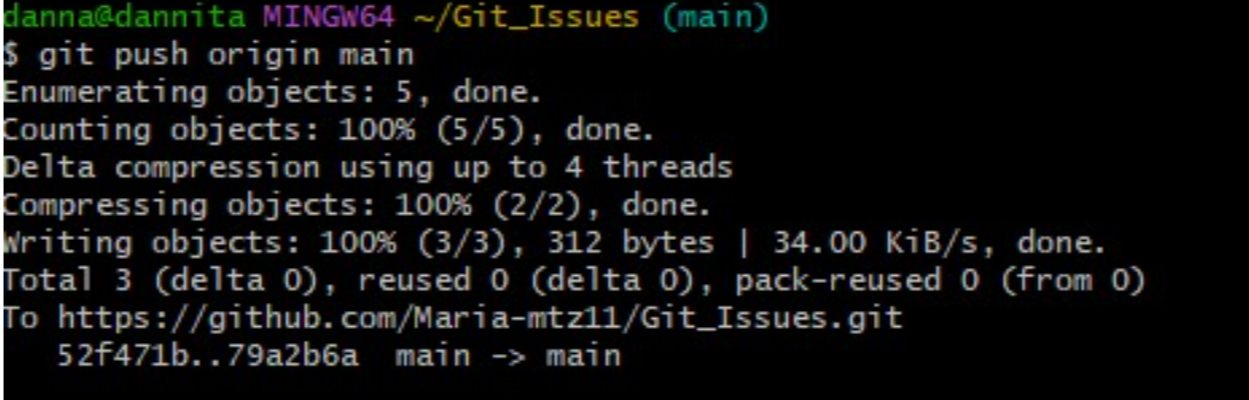
\includegraphics[width=0.9\textwidth]{imagenes/cambios.png}
\caption{Envío de los cambios al repositorio remoto mediante Git Push.}
\label{fig:cambios}
\end{figure}

\subsection{Cierre del Issue}

Una vez solucionado el problema, se procedió al cierre del Issue utilizando GitHub CLI.

\begin{lstlisting}[language=bash]
gh issue close 1
\end{lstlisting}

Con ello la incidencia quedó marcada como resuelta dentro del repositorio.

\begin{figure}[H]
\centering
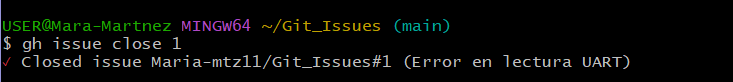
\includegraphics[width=0.9\textwidth]{imagenes/cierre.png}
\caption{Issue cerrado exitosamente.}
\label{fig:cierre}
\end{figure}